\documentclass{article}
\graphicspath{{/home/david/Book/Chapters/1.Revision/LinearEquation/pic/}}

% !TeX root = ../../../Mainfile/book.tex



\begin{document}


\section{Linear equations}

\[
x + 2 = y 
\]


That was an example of a \textbf{linear equation}. 

It has two variables, $x$ and $y$, and it describes how the value of one of the variables depends on the value of the other variable.

Lets plot (draw) this equation for a few diferent values of $x$, like $-6$, $-2$, $1$ and $5$



\begin{figure}[h]
\centering
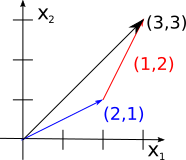
\includegraphics[scale = .30]{1.png}
\end{figure}

The graph of a linear equation is always a line 

\end{document}